\documentclass[border=5pt]{standalone}
\usepackage{tikz}
\usetikzlibrary{arrows.meta, positioning, calc}
\usepackage{amsmath}
\usepackage{graphicx}

\begin{document}
\begin{tikzpicture}[
    node distance=0.4cm,
    arr/.style={-{Stealth[length=2.5mm]}, thick, black!70},
    imgnode/.style={inner sep=0pt, outer sep=0pt},
    box/.style={draw, thick, rounded corners=2pt, fill=white, font=\scriptsize\bfseries, align=center, minimum height=0.8cm, minimum width=1.8cm},
  ]

  % ============ TOP ROW (main pipeline) ============

  % ---- 1. Flightmare ----
  \node[imgnode] (sim) {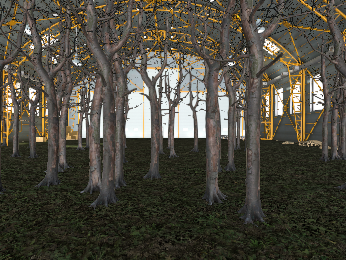
\includegraphics[width=2.4cm]{Flightmare.png}};
  \node[above=0.1cm of sim, font=\scriptsize\bfseries] {Flightmare Simulator};

  % ---- 2. Grayscale frames (stacked) ----
  \node[imgnode, right=1.4cm of sim] (gs_back) {%
    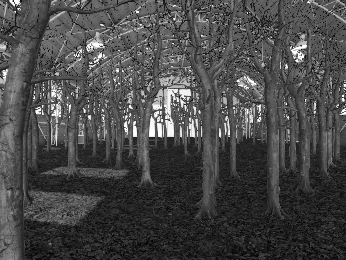
\includegraphics[width=2.0cm]{grayscale_I_t2.png}};
  \node[imgnode, shift={(-0.15cm,0.15cm)}] at (gs_back.center) (gs_front) {%
    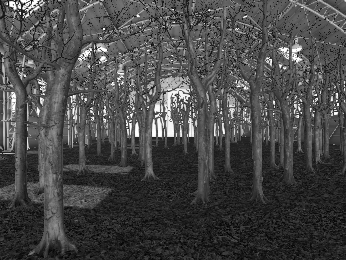
\includegraphics[width=2.0cm]{grayscale_I_t1.png}};
  \node[above=0.4cm of gs_front, font=\scriptsize\bfseries] {Grayscale Frames};
  \node[above=0.1cm of gs_front, font=\tiny] {$(I_{t_1}, I_{t_2})$};

  % ---- 3. Log-Difference ----
  \node[imgnode, right=1.4cm of gs_back] (logdiff) {%
    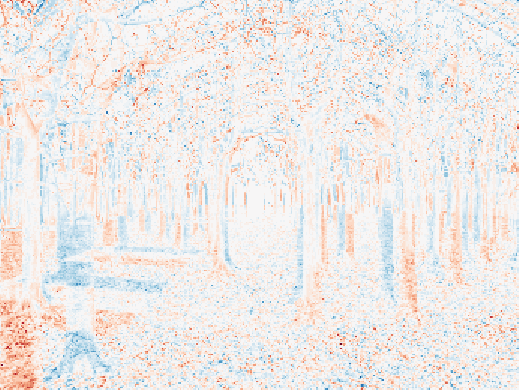
\includegraphics[width=2.0cm]{logdiff_vis.png}};
  \node[above=0.4cm of logdiff, font=\scriptsize\bfseries] {Log-Difference};
  \node[above=0.1cm of logdiff, font=\tiny] {$\Delta L(x,y)$};

  % ---- 4. 2-Channel Polarity ----
  \node[imgnode, right=1.4cm of logdiff] (pol) {%
    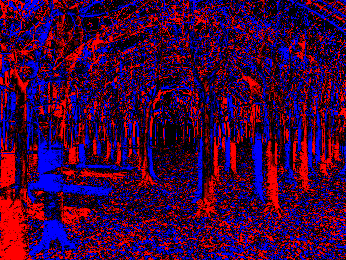
\includegraphics[width=2.0cm]{2-ch_vis.png}};
  \node[above=0.4cm of pol, font=\scriptsize\bfseries] {2-Ch Polarity};
  \node[above=0.1cm of pol, font=\tiny] {$(e^{-}, e^{+})$};

  % ---- 5. U-Net (simplified U-shape) ----
  \coordinate (unet_anchor) at ($(pol.east)+(2.2cm,0)$);
  \begin{scope}[shift={(unet_anchor)}]
    % Encoder bars (left side, getting shorter)
    \fill[orange!60] (-0.6, 0.5)  rectangle (-0.45, -0.5);
    \fill[orange!70] (-0.35, 0.4) rectangle (-0.2, -0.4);
    \fill[orange!80] (-0.1, 0.3)  rectangle (0.05, -0.3);

    % Bottleneck
    \fill[red!60] (0.15, 0.2) rectangle (0.3, -0.2);

    % Decoder bars (right side, getting taller)
    \fill[blue!50] (0.4, 0.3)  rectangle (0.55, -0.3);
    \fill[blue!40] (0.65, 0.4) rectangle (0.8, -0.4);
    \fill[blue!30] (0.9, 0.5)  rectangle (1.05, -0.5);

    % Skip connection arrows (curved)
    \draw[gray, thin, dashed, -{Stealth[length=1.5mm]}] (-0.52, 0.45) to[bend left=40] (0.97, 0.45);
    \draw[gray, thin, dashed, -{Stealth[length=1.5mm]}] (-0.27, 0.35) to[bend left=35] (0.72, 0.35);
    \draw[gray, thin, dashed, -{Stealth[length=1.5mm]}] (-0.02, 0.25) to[bend left=30] (0.47, 0.25);

    % Label (above)
    \node[font=\scriptsize\bfseries, above] at (0.225, 0.55) {U-Net Depth Estimator};
  \end{scope}

  \coordinate (unet_in) at ($(unet_anchor)+(-0.7cm,0)$);
  \coordinate (unet_out) at ($(unet_anchor)+(1.15cm,0)$);
  \coordinate (unet_top) at ($(unet_anchor)+(0.225cm,0.55cm)$);
  \coordinate (unet_bot) at ($(unet_anchor)+(0.225cm,-0.5cm)$);

  % ---- 6. Predicted Depth ----
  \node[imgnode, right=2.4cm of unet_out] (pred) {%
    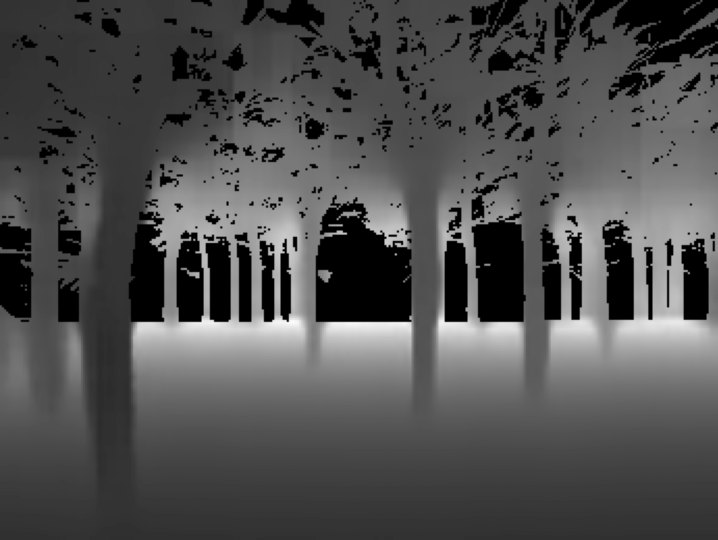
\includegraphics[width=2.0cm]{pred_depth.png}};
  \node[above=0.4cm of pred, font=\scriptsize\bfseries] {Predicted Depth};
  \node[above=0.1cm of pred, font=\tiny] {$\hat{D}$};

  % ============ BOTTOM SECTION ============

  % ---- Loss node (below Predicted Depth) ----
  \node[box, minimum width=2.4cm, below=1.8cm of pred] (loss) {%
    Loss\\[-1pt]
    {\tiny $(\mathcal{L}_{\text{BerHu}} + \lambda_g \cdot \mathcal{L}_{\text{grad}})$}};

  % ---- Ground Truth (below Loss) ----
  \node[imgnode, below=1.0cm of loss] (gt) {%
    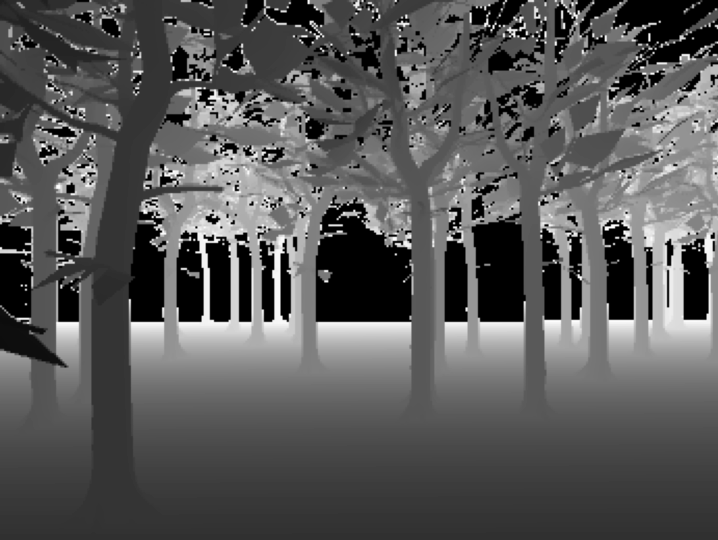
\includegraphics[width=2.0cm]{ground_truth.png}};
  \node[below=0.1cm of gt, font=\scriptsize\bfseries] {Ground Truth};
  \node[below=0.4cm of gt, font=\tiny] {$D$};

  % ---- CMA-ES box (right of Loss) ----
  \node[box, fill=yellow!15, right=1.8cm of loss] (cmaes) {%
    CMA-ES\\[-1pt]
    {\tiny $(\eta,\;\alpha,\;\lambda_g)$}};

  % ============ ARROWS ============

  % Top row: left to right pipeline
  \draw[arr] (sim.east) -- (gs_back.west);
  \draw[arr] (gs_back.east) -- (logdiff.west);
  \draw[arr] (logdiff.east) -- (pol.west);
  \draw[arr] (pol.east) -- (unet_in);
  \draw[arr] (unet_out) -- (pred.west);

  % Predicted Depth straight down to Loss
  \draw[arr] (pred.south) -- (loss.north);

  % GT up to Loss
  \draw[arr] (gt.north) -- (loss.south);

  % Loss right to CMA-ES with val_MAE label below and Tune label below that
  \draw[arr] (loss.east) -- node[above, font=\tiny\bfseries] {val\_MAE} node[below, font=\tiny\bfseries] {Tune} (cmaes.west);

  % Training loop: Loss → left → up → into U-Net bottom (Train label below arrow)
  \coordinate (train_corner) at (unet_bot |- loss);
  \draw[arr] (loss.west) -- node[below, font=\tiny\bfseries] {Train} (train_corner) -- (unet_bot);

  % Tuning loop: CMA-ES → up above labels → left → down into U-Net top
  % Go 1.2cm above the U-Net label to clear everything
  \coordinate (tune_height) at ($(unet_top)+(0,1.6)$);
  \coordinate (tune_above_right) at (cmaes |- tune_height);
  \coordinate (tune_above_left) at (unet_top |- tune_height);
  \draw[arr] (cmaes.north) -- (tune_above_right) -- (tune_above_left) -- (unet_top);

\end{tikzpicture}
\end{document}
